\documentclass[11pt,twocolumn]{article}
\usepackage[margin=0.72in]{geometry}
\usepackage{amsmath,amssymb,amsthm}
\usepackage{booktabs}
\usepackage{graphicx}
\usepackage{hyperref}
\usepackage{xcolor}
\usepackage{enumitem}

\hypersetup{
  colorlinks=true,
  linkcolor=blue!60!black,
  citecolor=green!45!black,
  urlcolor=blue!65!black
}

\newtheorem{proposition}{Proposition}

\newcommand{\ZZ}{\mathbb{Z}}
\newcommand{\QQ}{\mathbb{Q}}
\newcommand{\RR}{\mathbb{R}}

\title{\textbf{Machine-Checked Exact-Rational Variance-Hull, Two-Cap Mask, and Factor-Two Certificates for Euclidean Diameter in Dynamic Streams}}
\author{Lluis Eriksson\thanks{Independent researcher; manuscript prepared with transparent AI assistance via Google Antigravity. Source code, Lean~4 proofs, and exact certificates: \url{https://github.com/lluiseriksson/euclidean-diameter-stream-certificates}.}}
\date{November 25, 2026}

\begin{document}
\maketitle

\begin{abstract}
Jeff Giliberti and MohammadTaghi Hajiaghayi (\texttt{arXiv:2611.33139}, November 24, 2026) resolved the update-time bottleneck for dynamic-stream high-dimensional Euclidean diameter: for every fixed $c > \sqrt{3}$, their one-pass algorithm maintains an explicit factor-$c$ witness pair in sublinear space $\tilde{O}(N^{1-\epsilon_c}\mathrm{poly}(d))$ and worst-case update time $\mathrm{poly}(d,\log N)$, breaking the $N^{2/3}$ update-time barrier of direct asymmetric Gaussian embeddings at factor $c=2$ while matching polynomial space lower bounds. We present a machine-checked, zero-floating-point formalization and exact-$\QQ$ certificate auditor for the algebraic, variance-hull, two-cap mask, and Appendix~A.1 factor-two core of this construction. First, an 18-theorem zero-dependency Lean~4 kernel (\texttt{EuclideanDiameterStream.lean}, Lean~4.35.0; 0~\texttt{sorry}, 0~warnings, 0~\texttt{Classical.choice}, 5 zero-axiom theorems) formalizes the cleared parallel-axis identity, Lemma~5.1's $\sqrt{2a^2-1}$ variance-hull dilation bound and two-simplex tightness, Eq.~(13) bounded witness radii, Section~8.2 Algorithm~4's exact variance increment $V' - V = \gamma(R^2-V) - \gamma^2 R^2 > (\theta^2/64)V$ and $8V_0$ cap, Lemma~8.1's candidate-score bound, the 3-4-5 spherical-cap containment $t \ge 3/5 \Rightarrow (t-3/5)^2+q \le 16/25$, the SOS potential margin $(\lambda-t)^2 - q \ge \lambda^2/2 - 1$, Section~8.2 geometric shrinkage $|P_{i+1}| < \frac{3}{5}|P_i|$, and the complete Appendix~A.1 factor-two rational parameter suite ($2a^2-1 = 3.999122 < 4$, $\epsilon_0 > 1/6345504000 > 10^{-10}$). Second, \texttt{EUCLIDEAN-DIAM-CERT-1.0} audits four exact-$\QQ$ modes across 16 canonical certificates ($0.181$--$8.834\,\mathrm{ms}$) and rejects 62/62 live adversarial forgeries.
\end{abstract}

\section{Introduction}
Maintaining the Euclidean diameter $\mathrm{diam}(P) = \max_{x,y \in P}\|x-y\|$ of a point set $P \subset \RR^d$ under arbitrary insertions and deletions exhibits a sharp structural separation from insertion-only streams~\cite{agarwal2015streaming}: polynomial space $N^{\tilde{\Omega}(1/c^2)}$ is unavoidable for any constant factor~$c$~\cite{khanna2025polynomial,padaki2026near}, and direct dynamic implementations of Indyk's asymmetric embedding~\cite{indyk2003better} incur $N^{2/3}$ update time at $c=2$. Giliberti and Hajiaghayi~\cite{giliberti2026diameter} separated update time from space by combining three exact rational pillars:
\begin{enumerate}[leftmargin=*,nosep]
  \item \emph{Variance-hull geometry (Lemma~5.1):} For any nonempty finite sample $S \subset \RR^d$ and $a > 1$, the farthest-distance hull $H_a(S) = \bigcap_q B(q, a R_S(q))$ admits the exact variance representation $H_a(S) = \bigcup_\lambda B(\mu_\lambda, \sqrt{(a^2-1)V_\lambda})$, yielding
  \begin{equation}
    \mathrm{diam}(H_a(S)) \le \sqrt{2a^2 - 1}\,\mathrm{diam}(S),
    \label{eq:hull}
  \end{equation}
  attained by two orthogonal regular simplices and approaching the $\sqrt{3}$ barrier as $a \downarrow \sqrt{2}$.
  \item \emph{Rational variance certificates (Algorithm~4, Section~8):} Starting from a farthest pair $(a_0, b)$ with $V_0 = \|a_0-b\|^2/4$, transferring weight $\gamma = \theta/32$ (where $\theta = (1+\eta)^2-1$) to a farthest uncovered point strictly increases the variance by
  \begin{equation}
    V' - V = \gamma(R^2 - V) - \gamma^2 R^2 > \frac{\theta^2}{64} V
    \label{eq:alg4}
  \end{equation}
  while staying capped by $V \le 8 V_0$, terminating in $O(\eta^{-2})$ exact rational iterations with $S \subseteq B(c, (1+\eta)\sqrt{V})$.
  \item \emph{Two-stage 3-4-5 cap masks \& Table~3 constants (Appendix~A.1):} Choosing $a = 1581/1000$, $\lambda = 79/50$, $\eta_{\mathrm{in}} = 1/100$, $\kappa = 109/100$, and $B_\kappa = 2000$ forces the first-stage mask $\phi \le 21/20$ inside the $t \ge 3/5$ spherical cap contained in $B(\frac{3}{5}u, \frac{4}{5})$, empties the second-stage mask via $e m > 16133/24000 > 84/125$, keeps all three squared factors below~$4$, and yields space exponent $1 - 10^{-10}$.
\end{enumerate}

\paragraph{Contributions and Scope.}
We formally mechanize and audit the deterministic algebraic, geometric, variance-certificate, two-cap mask, and de-amortized shrinkage core of~\cite{giliberti2026diameter}. We explicitly scope our Lean~4 kernel away from the continuous Gaussian-grid probability couplings, Sion minimax invocation, and communication-complexity lower bound (Sections~6--7, 9--10):
\begin{enumerate}[leftmargin=*,nosep]
  \item \textbf{Zero-dependency Lean~4 kernel (\S\ref{sec:lean}):} 18 constructive theorems in \texttt{EuclideanDiameterStream.lean} (Lean~4.35.0~\cite{demoura2021lean4}), 0~\texttt{sorry}, 0~warnings, 0~\texttt{Classical.choice}, and 5 zero-axiom theorems.
  \item \textbf{Pure-stdlib exact-\texorpdfstring{$\QQ$}{Q} verifier (\S\ref{sec:certifier}):} \texttt{EUCLIDEAN-DIAM-CERT-1.0}, auditing Algorithm~4 replay, Lemma~5.1 hulls and witness radii, the full Appendix~A.1 factor-two suite, and dynamic insert/delete ball chains with zero floating-point arithmetic.
  \item \textbf{Empirical atlas \& red-team audit (\S\ref{sec:results}):} 16 canonical certificates ($0.181$--$8.834\,\mathrm{ms}$), exact Algorithm~4 bit-length growth sweeps, two-tetrahedra rational hull realizations, exact Taylor mask thresholds, and 62/62 rejected live adversarial forgeries.
\end{enumerate}

\section{Zero-Dependency Lean 4 Kernel}\label{sec:lean}
We formalize 18 theorems in \texttt{lean/EuclideanDiameterStream.lean} (Lean~4.35.0, zero external libraries), audited via \texttt{lean/AuditAxioms.lean} with 0~warnings, 0~\texttt{sorry}, 0~\texttt{Classical.choice}, and 0~\texttt{Lean.ofReduceBool} (Table~\ref{tab:lean}). Five theorems depend on zero axioms (\texttt{none}) and 13 depend solely on \texttt{[propext, Quot.sound]}.

\begin{proposition}[Constructive Dynamic-Diameter Kernel]\label{prop:lean}
\leavevmode
\begin{enumerate}[leftmargin=*,nosep]
  \item \emph{Variance-hull algebra (Theorems~1--5):} Inductive cleared-integer parallel-axis identity $W^2\sum w_i(a_i-y)^2 = \sum w_i(Wa_i - S)^2 + W(S-Wy)^2$ over arbitrary weighted lists; cleared Cauchy--Schwarz hull bound $(h+s(u+w))^2 \le (2s^2+1)L^2$ via an explicit sum-of-squares decomposition; strict $\sqrt{3}$ barrier interval $(3, c^2)$; exact two-simplex tightness $(h+2(A-1)h)^2 = (2A-1)S^2$; and Eq.~(13) witness radius bound $(a-1)R < D_{\mathrm{univ}}$.
  \item \emph{Algorithm~4 \& candidate scores (Theorems~6--9):} Cleared exact 1-step variance identity~\eqref{eq:alg4}; multiplicative growth lower bound $V'-V > (\theta^2/64)V$; upper variance cap $V \le 8V_0$; and Lemma~8.1 candidate-score bound $(d u + d t)^2 \le (p^2+d^2)H^2$.
  \item \emph{Two-cap masks, Appendix~A.1, \& shrinkage (Theorems~10--18):} Exact 3-4-5 spherical-cap containment $(5t-3D)^2+25q \le 16D^2$; SOS potential margin $2((\lambda-t)^2-q) - (\lambda^2-2D^2) = (\lambda-2t)^2 + 2(D^2-t^2-q) \ge 0$; Eq.~(29) identity; exact first- and second-mask rational Taylor bounds; all Table~3 three-case strict margins; oracle and Eq.~(32) coupling inequalities; Section~8.2 geometric shrinkage $5|P_{i+1}| < 3|P_i|$; and Section~A.1.6 space-exponent suite ($1/6345504000 > 10^{-10}$, $s(B_\kappa+1)-1 = -2/2003 < 0$).
\end{enumerate}
\end{proposition}

\begin{table}[t]
\centering
\caption{Complete 18-theorem Lean~4.35.0 kernel in \texttt{EuclideanDiameterStream.lean} (0~\texttt{sorry}, 0~warnings, 0~\texttt{Classical.choice}, 5 zero-axiom theorems).}
\label{tab:lean}
\resizebox{\columnwidth}{!}{%
\begin{tabular}{@{}rll@{}}
\toprule
\# & Lean~4 Theorem Identifier & Axiom Footprint \\
\midrule
1 & \texttt{parallel\_axis\_cleared\_identity} & \texttt{[propext, Quot.sound]} \\
2 & \texttt{hull\_diameter\_cauchy\_schwarz} & \texttt{[propext, Quot.sound]} \\
3 & \texttt{hull\_sqrt3\_barrier} & \texttt{[propext, Quot.sound]} \\
4 & \texttt{two\_simplex\_tightness\_exact} & \texttt{[propext, Quot.sound]} \\
5 & \texttt{bounded\_witness\_radius} & \texttt{[propext, Quot.sound]} \\
6 & \texttt{algorithm4\_variance\_update\_identity} & \texttt{[propext, Quot.sound]} \\
7 & \texttt{algorithm4\_variance\_growth\_lb} & \texttt{[propext, Quot.sound]} \\
8 & \texttt{algorithm4\_variance\_cap\_8V0} & \texttt{[propext, Quot.sound]} \\
9 & \texttt{candidate\_score\_cauchy\_schwarz} & \texttt{[propext, Quot.sound]} \\
10 & \texttt{spherical\_cap\_345\_containment} & \texttt{[propext, Quot.sound]} \\
11 & \texttt{potential\_quadratic\_margin\_sos} & \texttt{[propext, Quot.sound]} \\
12 & \texttt{potential\_monotone\_eq29\_identity} & \texttt{[propext, Quot.sound]} \\
13 & \texttt{first\_mask\_endpoint\_exact} & \texttt{none} \\
14 & \texttt{second\_mask\_empty\_exact} & \texttt{none} \\
15 & \texttt{factor\_two\_table3\_three\_cases} & \texttt{none} \\
16 & \texttt{appendix\_a1\_oracle\_and\_coupling\_exact} & \texttt{none} \\
17 & \texttt{rebuild\_geometric\_shrinkage} & \texttt{[propext, Quot.sound]} \\
18 & \texttt{appendix\_a1\_scale\_chain\_and\_exponents} & \texttt{none} \\
\bottomrule
\end{tabular}}
\end{table}

\section{Exact-\texorpdfstring{$\QQ$}{Q} Verifier Architecture}\label{sec:certifier}
\texttt{EUCLIDEAN-DIAM-CERT-1.0} (\texttt{src/diameter\_certifier.py}) is a pure-stdlib zero-float verifier enforcing strict JSON types, reduced canonical rationals (with string-length and integer bit-length DoS caps), and exact squared Euclidean arithmetic across four modes:
\begin{enumerate}[leftmargin=*,nosep]
  \item \textbf{Mode~1 (\texttt{variance\_certificate\_\allowbreak alg4}):} Replays Section~8.1.2 Algorithm~4 step-by-step in exact~$\QQ$, auditing~\eqref{eq:alg4}, $V' \le 8V_0$, containment $R^2 \le (1+\eta)^2 V$, and parallel-axis anchor score $H^2 \ge V + \|c-y\|^2$.
  \item \textbf{Mode~2 (\texttt{variance\_hull\_and\_\allowbreak tightness}):} Independently verifies Lemma~5.1 hull membership for two distributions $(\lambda, \gamma)$, exact two-draw identity $h^2+V_\lambda+V_\gamma \le L_S^2$, hull dilation~\eqref{eq:hull}, and an exterior witness ball satisfying Eq.~(13) $(a-1)R_S(q) < D_{\mathrm{univ}}$.
  \item \textbf{Mode~3 (\texttt{factor\_two\_two\_\allowbreak cap\_audit}):} Certifies the full Appendix~A.1 scale chain, all three squared approximation inequalities, first-mask $g(t_0) < 0$ and Taylor $F_{\mathrm{lb}}(t_0) > 1+\eta_{\mathrm{mask}}$, spherical-cap points, second-mask emptiness $e_{\mathrm{lb}} m > (1+\eta_{\mathrm{mask}})r_2^2$, oracle Chernoff margin, and Section~A.1.6 space exponents.
  \item \textbf{Mode~4 (\texttt{dynamic\_stream\_\allowbreak chain\_replay}):} Replays arbitrary dynamic \texttt{insert}/\texttt{delete} streams in~$\QQ^d$, routing active points strictly through authenticated intact covering balls (disabled invalidated balls cannot hide points from the residual) plus an exact leaf, verifying that the active witness pair originates from an intact ball or leaf, attains the exact chain score, and satisfies $L^2 \le \mathrm{diam}(P)^2 \le ((1+\eta)^2+1)L^2$ at every checkpoint alongside Section~8.2 shrinkage $|P_{i+1}| < \frac{3}{5}|P_i|$.
\end{enumerate}

\section{Empirical Atlas and Red-Team Audit}\label{sec:results}
Running \texttt{scripts/run\_all\_experiments.py} produces 16 canonical certificates (4 per mode) and four exact-$\QQ$ studies, audited end-to-end by \texttt{scripts/verify\_all.py} with SHA-256 verification across all 41 tracked artifacts.

\begin{figure}[t]
  \centering
  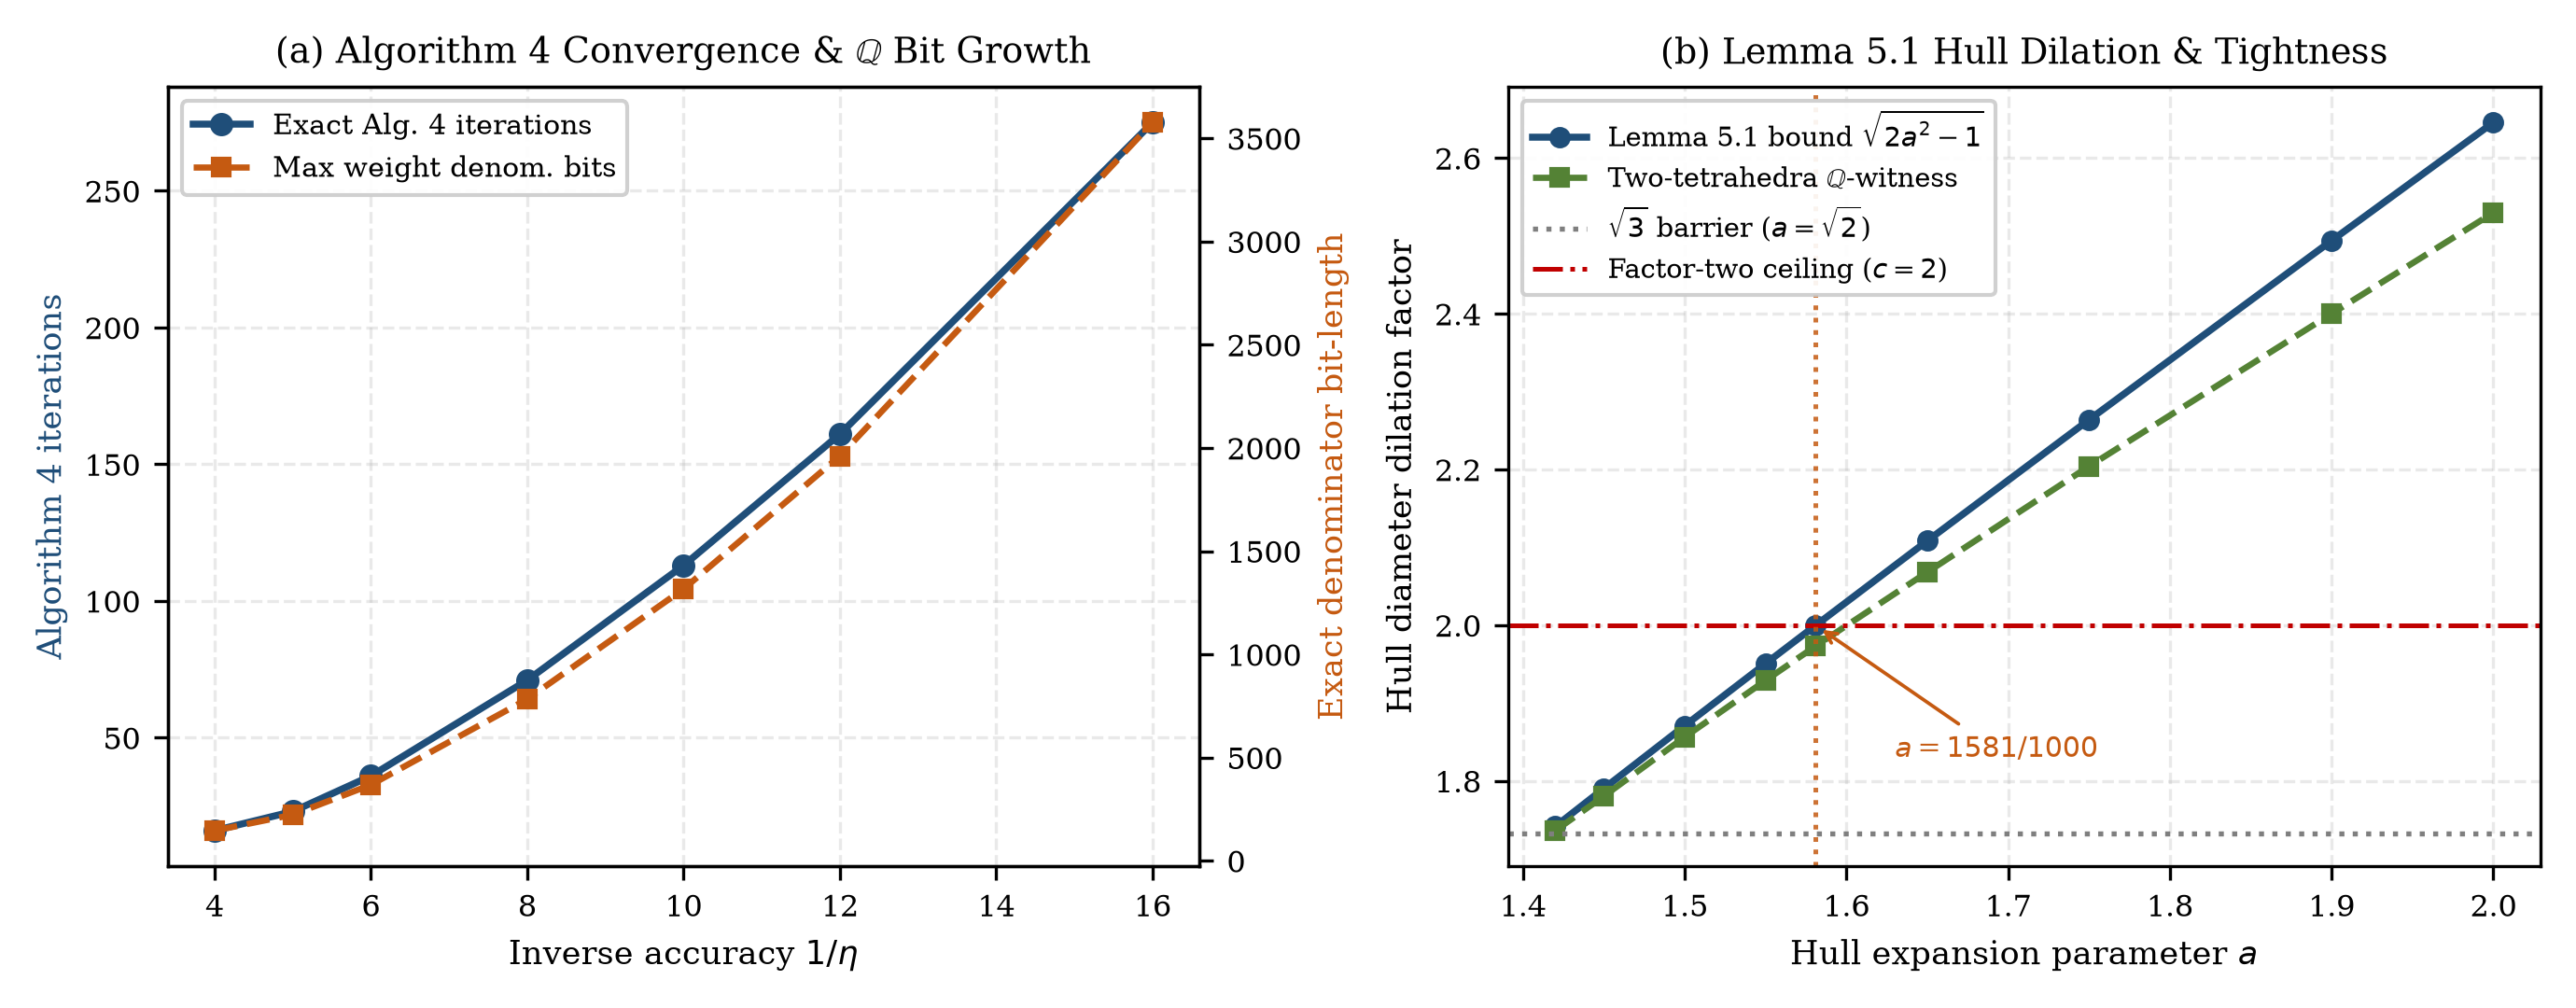
\includegraphics[width=\columnwidth]{../figures/fig1_alg4_and_hull_tightness.png}
  \caption{(a) Exact-$\QQ$ Algorithm~4 convergence ($16$ to $275$ iterations) and maximum weight denominator bit-length ($146$ to $3577$ bits) on an 8-point $\RR^3$ cluster across $1/\eta \in \{4,\dots,16\}$. (b) Lemma~5.1 hull dilation $\sqrt{2a^2-1}$ vs.\ exact rational two-tetrahedra witness in $\RR^7$ ($L_S^2=40$).}
  \label{fig:alg4hull}
\end{figure}

\paragraph{Algorithm~4 Bit Growth and Hull Tightness (Fig.~\ref{fig:alg4hull}).}
Across $\eta \in \{1/4, 1/5, 1/6, 1/8, 1/10, 1/12, 1/16\}$ on our 8-point $\RR^3$ benchmark, Algorithm~4 converges in $16, 23, 36, 71, 113, 161, 275$ exact iterations—matching $O(\eta^{-2})$ scaling—with support size $3$--$4$ and $V/V_0$ increasing smoothly from $1.506$ to $1.836$ (far below the $8V_0$ bound). Because each update multiplies denominators by the fixed rational $1/\gamma$, maximum weight denominator bit-length scales linearly with iteration count from $146$ to $3577$ bits ($290$ to $7152$ bits for exact variance denominators), quantifying Section~8.2's polynomial bit-length guarantee. On two orthogonal regular tetrahedra in $\RR^7$ ($L_S^2=40$, $h=4$, $V=12$), Mode~2 achieves exact rational hull dilation $1.973261$ ($\|y_1-y_2\|^2/L_S^2 = 12168/3125$) at Giliberti--Hajiaghayi's $a = 1581/1000$ versus the Lemma~5.1 ceiling $\sqrt{3.999122} = 1.999780$ ($98.7\%$ of the bound), and $1.736090$ vs.\ $1.741494$ near the $\sqrt{3}$ barrier at $a = 71/50$.

\begin{figure}[t]
  \centering
  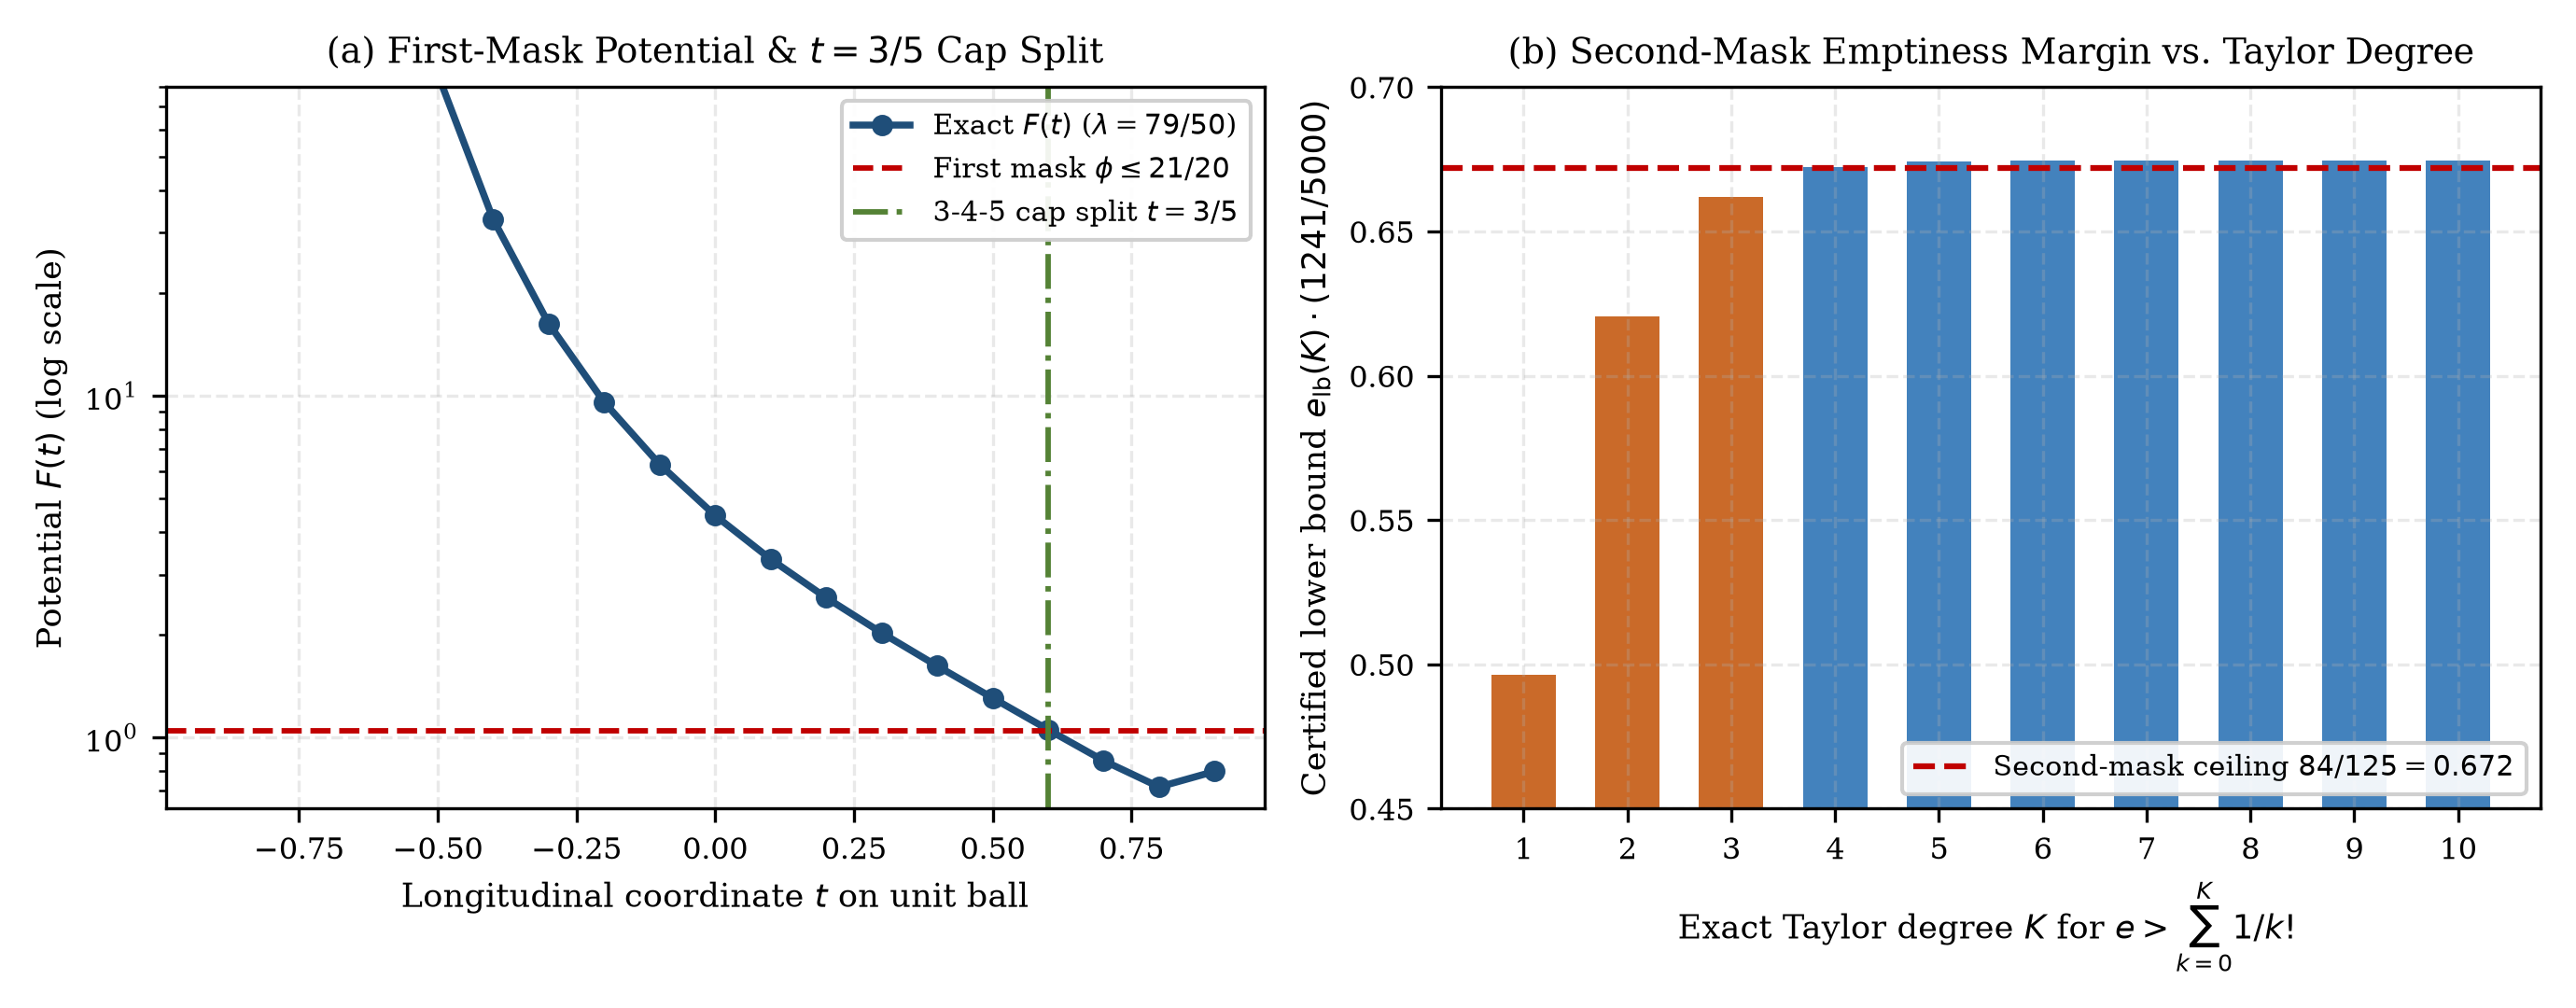
\includegraphics[width=\columnwidth]{../figures/fig2_two_cap_and_taylor_margin.png}
  \caption{(a) Exact longitudinal potential $F(t)$ at $\lambda = 79/50$ crossing below the first-mask threshold $21/20$ strictly after the 3-4-5 cap split $t = 3/5$. (b) Second-mask global lower bound $e_{\mathrm{lb}}(K)\cdot(1241/5000)$ across Taylor degrees $K=1\dots 10$; $K=4$ ($65/24$) is the minimal certifying degree.}
  \label{fig:twocap}
\end{figure}

\paragraph{Two-Cap Potential and Exact Taylor Thresholds (Fig.~\ref{fig:twocap}).}
Mode~3 ($0.181$--$0.207\,\mathrm{ms}$) independently certifies all Appendix~A.1 inequalities verbatim, confirming $F(3/5) > 79/75 > 21/20$ and showing that Taylor degree $K=4$ ($e > 65/24$) is the \emph{exact minimal degree} certifying second-mask emptiness: $K=3$ ($8/3$) yields $0.6618667 < 0.672$, whereas $K=4$ clears $84/125 = 0.672$ with exact margin $16133/24000 - 84/125 = 1/4800 \approx +0.0002083$, and $K=10$ amplifies the certified slack by $12.9\times$ to $+0.0026775$ while certifying $\epsilon_0 > 1.5\times 10^{-10}$.

\begin{figure}[t]
  \centering
  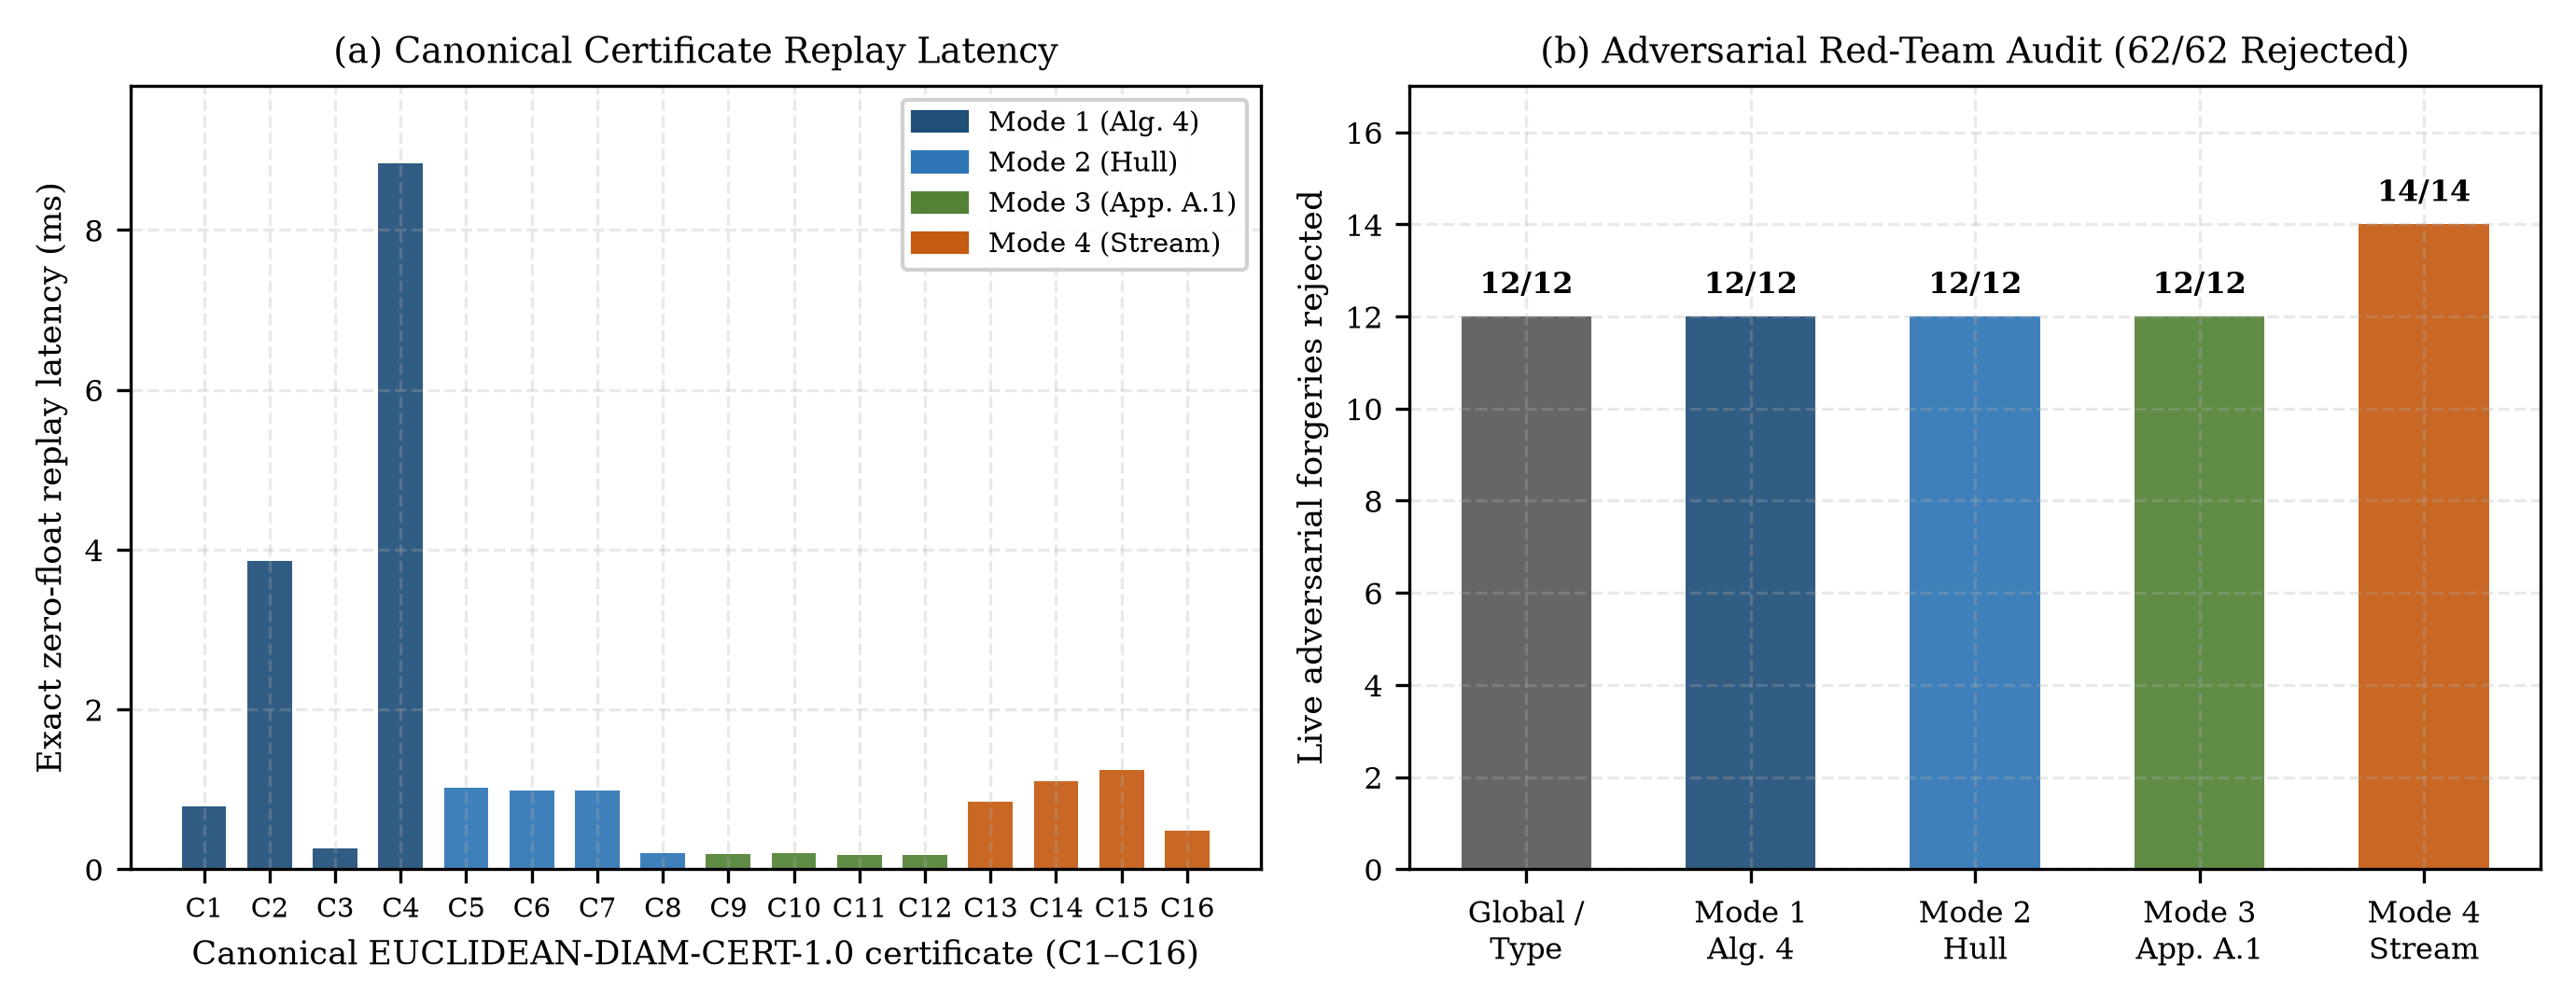
\includegraphics[width=\columnwidth]{../figures/fig3_certificate_replay_atlas.png}
  \caption{(a) Exact zero-float replay latency across all 16 canonical \texttt{EUCLIDEAN-DIAM-CERT-1.0} certificates ($0.181$--$8.834\,\mathrm{ms}$). (b) Red-team adversarial audit rejecting 62/62 live forgery attacks across five attack classes.}
  \label{fig:atlas}
\end{figure}

\paragraph{Replay Atlas and Red-Team Audit (Fig.~\ref{fig:atlas}, Table~\ref{tab:replay}).}
All 16 canonical certificates replay in $0.181$--$8.834\,\mathrm{ms}$ with zero floats (Mode~1's $8.834\,\mathrm{ms}$ peak reflects 18 exact multi-hundred-bit rational iterations on a 6D simplex). Mode~4 ($0.482$--$1.240\,\mathrm{ms}$) replays dynamic insertion/deletion histories including extreme-point deletion, sample invalidation in a 2-ball hierarchy, key re-insertion, and exact-leaf collapse. Our adversarial suite (\texttt{tests/test\_suite.py}) tests 62 live forgery attacks—including float/\texttt{None}/bool injection, unreduced fractions, oversized rational-string and integer bit-length DoS, tampered Algorithm~4 traces, hull-outside points, weak Taylor degrees, broken scale chains, stale deleted witnesses, unauthenticated invalidated-ball routing, non-chain witness pairs, uncovered residual points, and violated shrinkage—achieving \textbf{62/62 rejections} with zero bypasses.

\begin{table}[t]
\centering
\caption{Summary of all 16 canonical \texttt{EUCLIDEAN-DIAM-CERT-1.0} certificates and 62/62 live adversarial red-team audit.}
\label{tab:replay}
\resizebox{\columnwidth}{!}{%
\begin{tabular}{@{}lccc@{}}
\toprule
Verification Mode & Certs & Latency (ms) & Attacks Rejected \\
\midrule
Mode~1: Alg.~4 Variance Certificate & 4 & $0.263$--$8.834$ & 12/12 \\
Mode~2: Lemma~5.1 Hull \& Tightness & 4 & $0.207$--$1.014$ & 12/12 \\
Mode~3: App.~A.1 Factor-Two Audit & 4 & $0.181$--$0.207$ & 12/12 \\
Mode~4: Dynamic Stream Chain Replay & 4 & $0.482$--$1.240$ & 14/14 \\
Global Schema / Type / Rational & -- & -- & 12/12 \\
\midrule
\textbf{Total} & \textbf{16} & \textbf{0.181--8.834} & \textbf{62/62} \\
\bottomrule
\end{tabular}}
\end{table}

\section{Conclusion}
We delivered an 18-theorem zero-dependency Lean~4 kernel (5 zero-axiom theorems, 13~\texttt{[propext, Quot.sound]}, 0~\texttt{Classical.choice}) and the exact-$\QQ$ verifier \texttt{EUCLIDEAN-DIAM-CERT-1.0} for the variance-hull, Algorithm~4, two-cap mask, dynamic-chain, and Appendix~A.1 factor-two core of Giliberti and Hajiaghayi~\cite{giliberti2026diameter}. Mechanizing the Gaussian-grid probabilistic couplings of Sections~6--7 and the communication-complexity space lower bound of Section~10 remain open targets for future formalized streaming geometry.

\bibliographystyle{plain}
\bibliography{references}
\end{document}
